\documentclass[11pt,a4paper]{article}
\usepackage[T1]{fontenc}
\usepackage[utf8]{inputenc}
\usepackage{lmodern}
\usepackage[margin=1.05in]{geometry}
\usepackage{microtype}
\usepackage{amsmath,amssymb,amsthm,mathtools}
\usepackage{booktabs,tabularx}
\usepackage{graphicx}
\usepackage{enumitem}
\usepackage[backend=biber,style=numeric,sorting=none,natbib=true]{biblatex}
\addbibresource{references.bib}
\usepackage[hidelinks]{hyperref}
\usepackage[capitalise,nameinlink,noabbrev]{cleveref}

% Plain mathematical journal formatting: black text, numbered sections,
% centered title/author, abstract on first page, no ornamental title page.
\setlength{\parindent}{1.5em}
\setlength{\parskip}{0pt}
\setlength{\emergencystretch}{2em}
\pagestyle{plain}
\widowpenalty=10000
\clubpenalty=10000

\newtheorem{theorem}{Theorem}[section]
\newtheorem{proposition}[theorem]{Proposition}
\newtheorem{lemma}[theorem]{Lemma}
\theoremstyle{definition}
\newtheorem{definition}[theorem]{Definition}
\theoremstyle{remark}
\newtheorem{remark}[theorem]{Remark}
\DeclareMathOperator{\sgn}{sgn}
\DeclareMathOperator{\dist}{dist}
\DeclareMathOperator{\diam}{diam}
\newcommand{\Z}{\mathbb{Z}}
\newcommand{\G}{\mathcal{G}}
\newcommand{\C}{\mathcal{C}}
\newcommand{\moves}{\mathcal{S}}

\title{The Rubik's Cube as a Finite Group:\\
Permutations, Invariants, and Shortest-Path Search}
\author{Md Arif Hossain\\
\small Mathematics Graduate, Shahjalal University of Science and Technology\\
\small Sylhet, Bangladesh}
\date{}
\begin{document}
\maketitle
\begin{abstract}
The $3\times3\times3$ Rubik's Cube offers an unusually concrete route from elementary group theory to computational search. Its face turns generate a finite, non-abelian group whose elements correspond to the mechanically reachable configurations of the puzzle. This study develops the algebraic model from the group axioms and permutation composition, introduces a cubie-coordinate state representation, and derives the corner-orientation, edge-orientation, and permutation-parity constraints that characterize legal configurations. These invariants yield the well-known group order $43{,}252{,}003{,}274{,}489{,}856{,}000$. We then interpret optimal solving as a shortest-path problem on a Cayley graph and review the algorithmic significance of iterative-deepening A*, pattern databases, and subgroup-based two-phase methods. As a reproducible computational illustration, a breadth-first search using the restricted quarter-turn generators $U^{\pm1},R^{\pm1},F^{\pm1}$ enumerates $13{,}624$ configurations at distance at most six from the identity; invariants and move inverses are checked programmatically. This restricted experiment does \emph{not} calculate the complete cube diameter. The paper is expository in its established mathematical results and explicit about the limited originality of its computational demonstration, making it suitable as an independent technical study rather than as a claim of a novel theorem.
\end{abstract}
\noindent\textbf{Keywords:} finite groups; Rubik's Cube; permutation groups; invariants; Cayley graphs; computational algebra; breadth-first search; heuristic search.\\



\section{Introduction: from physical puzzle to mathematical object}
The Rubik's Cube is not only a speed-solving puzzle. It is a physical example of a finite transformation system: a state is changed by a small number of reversible operations, and the resulting transformations obey precise algebraic rules. That makes the cube a natural setting in which to study group actions, permutations, invariants, and algorithmic questions \citep{singmaster1981,joyner2008}.

The central distinction in this paper is between \emph{knowing how to perform a sequence of moves} and \emph{understanding the structure of the entire space of legal moves}. A human solving method often uses remembered sequences that preserve some solved pieces while moving others. The mathematics explains why such sequences work, why certain apparent cube arrangements are impossible, and why the definition of an optimal solution depends on how moves are counted.

This manuscript expands an earlier introductory treatment of the cube and group theory into a self-contained technical exposition. It addresses four questions:
\begin{enumerate}[leftmargin=*,itemsep=3pt]
\item What mathematical group is generated by the six basic face turns?
\item Which constraints distinguish legally reachable configurations from arbitrary reassemblies of the cubies?
\item How do shortest solutions correspond to distances in a graph?
\item What can a modest, reproducible search experiment demonstrate without making exaggerated claims about the full puzzle?
\end{enumerate}

The key established facts are credited to prior literature, including the cube-group treatment of \citet{joyner2008}, the pattern-database approach of \citet{korf1997}, and the computational diameter result of \citet{rokicki2013}. The computational exercise in \cref{sec:experiment} is a bounded verification and illustration, not an attempt to reproduce the computational proof of the full diameter.

\section{Related work and intellectual context}
\citet{singmaster1981} developed influential notation and an accessible language for recording cube transformations. \citet{joyner2008} presents a systematic mathematical treatment that connects the cube to groups, permutations, Cayley graphs, and legal versus illegal configurations. The cube also plays a role in algorithm design: \citet{korf1997} used iterative-deepening A* (IDA*) with pattern databases to compute optimal solutions for selected scrambled positions.

Two complementary directions followed. First, \citet{rokicki2013} established that the diameter of the standard $3\times3\times3$ cube group is exactly $20$ in the \emph{half-turn metric}. The proof combined subgroup cosets, symmetry reduction, and large-scale computation; the present paper does not independently verify that result. Second, \citet{demaine2011} studied algorithmic questions for generalized families of Rubik-type puzzles. Those asymptotic results must not be confused with a claim that the fixed $3\times3\times3$ cube is an NP-hard input family.

We also briefly explain the subgroup structure underlying Kociemba's two-phase method \citep{kociemba2phase}, which illustrates how an algebraically motivated change of state space can make search much more effective.

\section{Groups, permutations, and conventions}
\subsection{The group axioms}
\begin{definition}[Group]
A \emph{group} is a set $G$ equipped with a binary operation $\circ:G\times G\to G$ such that: (i) $a\circ b\in G$ for all $a,b\in G$; (ii) $(a\circ b)\circ c=a\circ(b\circ c)$; (iii) there exists an identity $e\in G$ satisfying $e\circ a=a\circ e=a$; and (iv) every $a\in G$ has an inverse $a^{-1}\in G$ satisfying $a\circ a^{-1}=a^{-1}\circ a=e$.
\end{definition}

A permutation of a finite set $X$ is a bijection $X\to X$. The set of all such permutations is the symmetric group $S_{|X|}$ under function composition. A cube move induces a permutation of visible moving facelets and, equivalently, a coordinated permutation and reorientation of its movable corner and edge cubies. Composition of legal moves is associative because composition of functions is associative.

Let $U,D,L,R,F,B$ denote clockwise $90^\circ$ rotations of the corresponding outer faces, from the perspective of looking toward the face. A prime denotes the inverse quarter-turn (for example $R^{-1}=R'$), while $R^2$ denotes a $180^\circ$ turn. These conventions are consistent with standard cube notation \citep{singmaster1981}.

\subsection{The cube group}
\begin{definition}[Rubik's Cube group]
Let $\G$ be the subgroup of permutations of the moving stickers generated by the six outer-face quarter turns:
\begin{equation}\label{eq:group}
\G=\langle U,D,L,R,F,B\rangle.
\end{equation}
The identity is the ``do nothing'' transformation, and multiplication corresponds to successive turns. We fix the reference orientation of the six center colors and distinguish configurations by their cubie positions and orientations.
\end{definition}

A face quarter-turn has inverse the counterclockwise turn and order four:
\begin{equation}
R^4=e,\qquad RR'=e,\qquad R^{-1}=R^3.
\end{equation}
Thus the group axioms can be checked directly from the underlying permutations. Importantly, the Rubik's Cube group is not abelian: $RU\neq UR$.

\subsection{An instructive commutator}
For group elements $a,b$, define their commutator by
\begin{equation}\label{eq:commutator}
[a,b]=aba^{-1}b^{-1}.
\end{equation}
The familiar move sequence $RUR'U'$ is an instance of $[R,U]$. If $R$ and $U$ commuted, this sequence would be the identity. They do not commute, and the result changes a subset of cubies. This construction suggests an important strategy: instead of solving an entire puzzle at once, one can build transformations that have relatively localized effects. Conjugates $gag^{-1}$ move the support of an operation $a$ to positions determined by $g$; this idea underlies many hand-designed cube algorithms \citep{joyner2008}.

\begin{proposition}
The move group $\G$ is non-abelian.
\end{proposition}
\begin{proof}
Consider the solved cube and the moves $R$ and $U$. Their associated permutations act on overlapping sets of corner positions. Directly tracking the upper-front-right corner under $RU$ and $UR$ shows two different final positions. Hence $RU\neq UR$, so not all group elements commute.
\end{proof}

\section{A cubie-coordinate representation}
A standard cube has eight movable corner cubies and twelve movable edge cubies; six center pieces establish the face-color reference. The movable cubies are most naturally represented by \emph{where they are} and \emph{how they are oriented}. Define the configuration vector
\begin{equation}\label{eq:state}
\C=(\sigma_c,\tau,\sigma_e,\phi),
\end{equation}
where $\sigma_c\in S_8$ is the corner permutation, $\tau\in\Z_3^8$ is the corner-twist vector, $\sigma_e\in S_{12}$ is the edge permutation, and $\phi\in\Z_2^{12}$ is the edge-flip vector. The orientation coordinates follow a consistent reference scheme (e.g. the cubie-coordinate convention in \citealp{kociemba2phase}).

The corner component is not arbitrary: corner twists are dependent modulo $3$. Likewise, the parity of the number of edge flips is restricted, and the edge/corner permutations cannot have independently chosen signs. These restrictions are not accidental implementation details; they are conserved properties of legal moves.

\subsection{How a face turn acts on the state}
A move $m$ can be stored as a position permutation $p_m$ together with orientation increments $t_m$ for corners, and analogously $q_m,f_m$ for edges. With the convention ``new position $k$ receives the cubie from old position $p_m(k)$,'' composition is
\begin{align}
\sigma'_c(k)&=\sigma_c(p_m(k)), & \tau'(k)&=\tau(p_m(k))+t_m(k)\pmod 3,\\
\sigma'_e(k)&=\sigma_e(q_m(k)), & \phi'(k)&=\phi(q_m(k))+f_m(k)\pmod 2.
\end{align}
The modulo operations encode the three possible corner orientations and two possible edge orientations. All computational results later in this manuscript use this representation and fixed move tables.

\section{Reachability invariants and legal configurations}
\subsection{Conservation of corner twist and edge flip}
\begin{lemma}[Orientation invariants]
For every state reachable by legal outer-face turns from the solved cube, the orientation coordinates satisfy
\begin{align}\label{eq:orientations}
\sum_{k=1}^{8}\tau_k&\equiv0\pmod 3,\\
\sum_{k=1}^{12}\phi_k&\equiv0\pmod 2.
\end{align}
\end{lemma}
\begin{proof}[Explanation]
Under any legal face move, the prescribed orientation changes have total corner twist congruent to zero modulo $3$ and total edge flip congruent to zero modulo $2$. The solved state satisfies both congruences. Because a finite sequence of moves is a composition of these invariant-preserving transformations, every reachable state also satisfies them. A complete treatment requires a fixed orientation convention; see \citet{joyner2008} and \citet{kociemba2phase}.
\end{proof}

Consequently, seven corner orientations can be selected independently, but the eighth is forced by the modulo-$3$ condition. Likewise, eleven edge flips can be selected independently, but the twelfth is determined by the modulo-$2$ condition. This rules out a single twisted corner or a single flipped edge created without disturbing anything else.

\subsection{Permutation parity}
The sign $\sgn(\sigma)\in\{+1,-1\}$ distinguishes even and odd permutations. A face quarter-turn induces a $4$-cycle of corners and a $4$-cycle of edges; each such cycle is odd. Therefore the parity of the corner permutation changes exactly when that of the edge permutation changes.

\begin{lemma}[Parity coupling]\label{lem:parity}
For every legally reachable cube configuration,
\begin{equation}\label{eq:parity}
\sgn(\sigma_c)=\sgn(\sigma_e).
\end{equation}
\end{lemma}
\begin{proof}
In the solved state both permutations are even. A face quarter-turn changes both permutation signs simultaneously. The equality is therefore preserved under every move and every move sequence.
\end{proof}

An isolated swap of exactly two edge cubies, with all other cubies fixed, violates \cref{eq:parity} and cannot be achieved by legal face turns.

\subsection{Characterizing the reachable states}
The three invariants above are not merely necessary. A standard cube-group theorem states that, for the usual fixed-center cubie representation, they are sufficient: any cubie arrangement satisfying the two orientation congruences and the matching-permutation-parity condition is realizable by a legal sequence. The sufficiency direction is nontrivial and is established in standard cube-group treatments; we do not present a new proof here \citep{joyner2008}.

\section{Counting the reachable configurations}
\begin{theorem}[Order of the standard cube group]\label{thm:order}
With fixed centers and the ordinary legal outer-face turns, the number of reachable configurations is
\begin{equation}\label{eq:order}
\boxed{|\G|=\frac{8!\,3^7\,12!\,2^{11}}{2}
=43{,}252{,}003{,}274{,}489{,}856{,}000.}
\end{equation}
\end{theorem}
\begin{proof}
There are $8!$ ways to permute the corners and $3^7$ admissible corner-orientation choices by \cref{eq:orientations}. There are $12!$ possible edge permutations and $2^{11}$ admissible edge orientations. Exactly half of the corner/edge permutation pairs have matching signs by \cref{eq:parity}. Multiplying the admissible independent choices yields \cref{eq:order}. The fact that every counted configuration is reachable follows from the sufficiency result cited in the preceding section.
\end{proof}

\begin{table}[htbp]
\centering
\caption{Components of the legal cube-state count.}
\label{tab:count}
\begin{tabular}{@{}p{.43\linewidth}p{.37\linewidth}@{}}
\toprule
\textbf{Component} & \textbf{Number of choices} \\
\midrule
Corner permutation & $8!=40{,}320$ \\
Corner orientations & $3^7=2{,}187$ \\
Edge permutation & $12!=479{,}001{,}600$ \\
Edge orientations & $2^{11}=2{,}048$ \\
Permutation-parity compatibility & factor $1/2$ \\
\midrule
\textbf{Total legal states} & $43{,}252{,}003{,}274{,}489{,}856{,}000$ \\
\bottomrule
\end{tabular}
\end{table}

For comparison, if arbitrary disassembly and reassembly allow every corner and edge orientation and position independently, the raw number of arrangements is
\begin{equation}
8!\,3^8\,12!\,2^{12}=519{,}024{,}039{,}293{,}878{,}272{,}000
=12|\G|.
\end{equation}
Hence only one in twelve such raw arrangements satisfies the legal constraints. This comparison counts labeled movable cubies and their orientations using fixed centers; counting whole-cube rotations as distinct would be a different convention and should not be silently mixed into the formula.

\section{Shortest paths and the Cayley graph}
\subsection{The graph model}
Let $\moves$ be a symmetric set of allowed moves, meaning $s\in\moves$ implies $s^{-1}\in\moves$. The corresponding Cayley graph $\operatorname{Cay}(\G,\moves)$ has one vertex for each cube state and an edge between $g$ and $gs$ for each $s\in\moves$. A solution to a scrambled cube $g$ is a path from $g$ to the identity $e$.

Define its minimum move count under the chosen move set by
\begin{equation}\label{eq:distance}
\ell_{\moves}(g)=\min\big\{k:g=s_1s_2\cdots s_k,\;s_i\in\moves\big\}.
\end{equation}
Then the worst-case optimal number of moves is the graph diameter
\begin{equation}\label{eq:diameter}
\diam\big(\operatorname{Cay}(\G,\moves)\big)
=\max_{g\in\G}\ell_{\moves}(g).
\end{equation}

\subsection{Move metrics matter}
The \emph{half-turn metric} (HTM) counts each $90^\circ$, $180^\circ$, or inverse $90^\circ$ face turn as one move, giving $18$ basic one-step choices. The \emph{quarter-turn metric} (QTM) counts a $180^\circ$ turn as two quarter turns. These distinct generating sets produce different graph distances.

The diameter in HTM is exactly $20$, as proved by \citet{rokicki2013}. The QTM diameter is exactly $26$, reported by \citet{qtm2014}. These results are outputs of much more extensive computational work than the limited experiment in this paper.

\section{Search algorithms and algebraic decomposition}
\subsection{Breadth-first search and exact short distances}
Breadth-first search (BFS) visits configurations in layers of increasing path length and therefore yields shortest paths when every move has unit cost. A naive BFS on the entire cube state space is infeasible for a modest desktop computer because the graph has more than $4\times10^{19}$ vertices. Nevertheless, a bounded BFS is useful for checking a representation, validating move inverses, and establishing exact distances within a small radius.

\subsection{IDA* and pattern databases}
For more demanding optimal search, IDA* combines depth-first expansion with an admissible heuristic $h(g)$ that never exceeds the true remaining distance. A pattern database stores precomputed exact distances in a projected state space. A valid lower bound on the complete state distance can be obtained from such a projected distance; several bounds may be combined by taking their maximum when they are individually admissible. \citet{korf1997} demonstrated the effectiveness of this general strategy for optimally solving selected cube instances.

\subsection{Two-phase subgroup search}
A complementary approach uses a well-chosen subgroup. In Kociemba's two-phase method, phase one searches for a transformation into
\begin{equation}\label{eq:phasegroup}
H=\langle U,D,R^2,L^2,F^2,B^2\rangle,
\end{equation}
whose states satisfy specialized orientation and slice-position conditions. Phase two then solves the remaining state while using moves that keep the cube inside $H$ \citep{kociemba2phase}. The significance is conceptual: using group structure changes the search problem into a sequence of smaller coordinate problems. The standard two-phase method aims at short solutions and is not, by itself, a guarantee of global optimality for every individual cube position.

\section{A reproducible bounded-search experiment}\label{sec:experiment}
\subsection{Aim and scope}
To complement the mathematical exposition, a compact state-space experiment was implemented in Python. Its purpose is to test the cubie representation and show how a finite group can be explored algorithmically. The generator set is deliberately restricted to
\begin{equation}
\moves_0=\{U,U',R,R',F,F'\},
\end{equation}
with each quarter-turn assigned unit cost. This is \emph{not} the complete six-face cube move set and is not an attempt to estimate the full HTM or QTM diameter.

The implementation stores four immutable tuples corresponding to \cref{eq:state}, uses the exact cubie move tables for $U,R,F$, constructs inverse moves by cubing each quarter-turn, and enumerates previously unseen states by BFS. The full executable program and machine-readable results are supplied in the companion archive.

\subsection{Algorithm and checks}
\begin{enumerate}[leftmargin=*,itemsep=3pt]
\item Initialize the frontier with the solved state $e$ and the visited set with $\{e\}$.
\item For each state in the current frontier, apply every move from $\moves_0$.
\item Retain only states not yet reached in an earlier layer; the resulting set forms the next frontier.
\item Record the frontier size and cumulative number of states, repeating through depth $6$.
\item Independently test that $U^4=R^4=F^4=e$, that the computed inverse of each move undoes it, and that every visited state satisfies both orientation invariants and the permutation-parity condition.
\end{enumerate}

Because BFS uses a visited set and unit-cost edges, every reported layer counts distinct states whose minimum distance from $e$, in this restricted graph, is exactly that layer index. The finite-depth calculation does not imply that unvisited states are unreachable.

\subsection{Results}
\begin{table}[htbp]
\centering
\caption{Distinct cube states found by BFS under $U^{\pm1},R^{\pm1},F^{\pm1}$. The counts are reproducible from the accompanying code.}
\label{tab:bfs}
\begin{tabular}{@{}rrr@{}}
\toprule
\textbf{Exact distance $d$} & \textbf{New states at $d$} & \textbf{Cumulative states}\\
\midrule
0 & 1 & 1\\
1 & 6 & 7\\
2 & 27 & 34\\
3 & 120 & 154\\
4 & 534 & 688\\
5 & 2,376 & 3,064\\
6 & 10,560 & 13,624\\
\bottomrule
\end{tabular}
\end{table}

\begin{figure}[htbp]
\centering
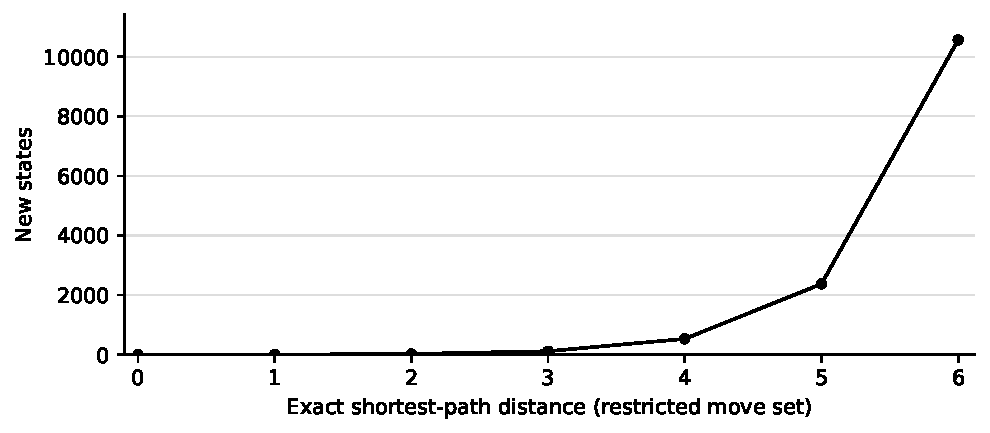
\includegraphics[width=.92\linewidth]{figures/bfs_growth.pdf}
\caption{Observed growth of distinct states at each exact shortest-path distance under the restricted six-generator quarter-turn move set. This is an enumeration through depth six, not the global cube distance distribution.}
\label{fig:growth}
\end{figure}

All $13{,}624$ visited configurations satisfy the corner-twist, edge-flip, and parity constraints. The program also verifies that the three face-quarter-turn generators have order four and that each generated inverse undoes the corresponding turn. Applying the commutator $RUR'U'$ to the solved configuration changes four corner cubies (counting position and orientation changes) and three edge cubies (counting position and orientation changes), under the implementation's cubie-coordinate convention.

The layer counts illustrate why systematic search quickly becomes expensive: branching generates many candidate sequences, and duplicate-state detection is necessary to avoid falsely treating different move sequences as different configurations. They also show the value of algebraic validation: an implementation bug in the move tables could produce a plausible-looking but incorrect search tree without the invariant checks.

\subsection{Reproducibility and limitations}
The companion file \texttt{code/cubie\_experiment.py} uses Python's standard library and no external cube-solver package. It can be rerun with
\begin{center}
\texttt{python code/cubie\_experiment.py --depth 6 --out code/results.json}
\end{center}
The reported integers are exact for the specified program, model, generator set, and BFS depth. The experiment does not prove that the move tables model every possible physical cube convention, does not provide a full solver, and does not establish any new complexity or diameter bound. More extensive tests and independent implementations would be needed for a stronger software-verification claim.

\section{Discussion: mathematical reasoning and computational search}
The Rubik's Cube illustrates a useful progression. A physical operation first becomes a permutation; sequences of reversible permutations become a group; simple conserved quantities restrict the legal state space; and the resulting finite group becomes a graph on which shortest-path methods can operate. Each step changes the nature of the question and offers a different form of explanation.

The invariants have immediate practical meaning. If a cube is reassembled with one flipped edge, a solver that searches only legal face-turn sequences will never succeed because the target is not in the same reachable component under those moves. The failure is a mathematical impossibility, not a deficiency in the solver's speed. Likewise, a valid arrangement may nevertheless require a long move sequence under a chosen metric, which motivates heuristic search and subgroup decomposition.

The same combination of mathematical formulation, feasibility checking, and search discipline is relevant to broader optimization problems: a plan should not merely look plausible, but must satisfy explicit constraints; a feasible solution is not necessarily optimal; and computational claims require a specified model and independent verification. This analogy is methodological rather than a claim that cube-solving and industrial scheduling are the same problem.

\section{Limitations and directions for further work}
The current paper is a rigorous \emph{expository and computational} manuscript. The principal theoretical facts (group structure, state count, reachability criteria, and graph diameters) are already known in the literature. Its added contribution is the reorganized treatment, corrected derivations, transparent conventions, and executable bounded-search illustration. It should not be described as a new theorem or as a peer-reviewed publication.

Possible extensions include: (i) independent comparison of multiple cubie-coordinate implementations; (ii) an exact shortest-path study for carefully chosen smaller subgroups; (iii) stronger experiments comparing BFS and admissible-heuristic A* on identical benchmark sets; (iv) analysis of the impact of symmetry reductions on explored states; and (v) a reproducible investigation of commutator-based solution construction. Each future extension should specify hypotheses, data, computational costs, and verification criteria in advance.

\section{Conclusion}
The Rubik's Cube provides a coherent bridge between abstract algebra and computational methods. With fixed center colors, its legal configurations form a finite non-abelian group of order $43{,}252{,}003{,}274{,}489{,}856{,}000$. Three simple reachability constraints---corner-twist conservation, edge-flip conservation, and matching corner/edge permutation parity---explain the dramatic reduction from all mechanically conceivable cubie arrangements to legal states. A Cayley-graph viewpoint translates solving into shortest-path search, where move metrics and algorithmic assumptions are crucial. The bounded BFS exercise demonstrates the mechanics of representation, invariant checking, and exact-distance enumeration on a small neighborhood of the solved state. The broader lesson is that mathematical structure and computational verification are strongest when used together, with precise distinctions between established results and the claims supported by a new experiment.

\appendix
\section{Notation and assumptions at a glance}
\begin{table}[h!]
\centering
\caption{Symbols used throughout the paper.}
\begin{tabularx}{\linewidth}{@{}lX@{}}
\toprule
Symbol & Meaning\\\midrule
$\G$ & Cube group generated by all six outer-face quarter turns.\\
$S_n$ & Symmetric group on $n$ labeled objects.\\
$\sigma_c,\sigma_e$ & Corner and edge position permutations.\\
$\tau\in\Z_3^8$ & Corner-twist coordinates.\\
$\phi\in\Z_2^{12}$ & Edge-flip coordinates.\\
$\moves$ & Symmetric set of allowed face turns; determines the move metric.\\
$\ell_{\moves}(g)$ & Minimum length of a word representing $g$ over the generating set $\moves$.\\
$\sgn(\sigma)$ & Permutation sign $\pm1$.\\
$H$ & Intermediate subgroup used in Kociemba-style two-phase search.\\
\bottomrule
\end{tabularx}
\end{table}

\section{Reproducible search pseudocode}
\begin{quote}\small\ttfamily
visited $\leftarrow$ \{identity\}\\
frontier $\leftarrow$ \{identity\}\\
for depth in 1,...,6:\\
\hspace*{1em} next $\leftarrow$ empty set\\
\hspace*{1em} for state in frontier:\\
\hspace*{2em} for move in \{U,U',R,R',F,F'\}:\\
\hspace*{3em} candidate $\leftarrow$ apply(state,move)\\
\hspace*{3em} if candidate not in visited: add candidate to next\\
\hspace*{1em} visited $\leftarrow$ visited union next\\
\hspace*{1em} frontier $\leftarrow$ next\\
\hspace*{1em} record |frontier| and |visited|
\end{quote}
The complete executable source is included in the accompanying project archive, together with the exact output file and the figure-generation script.

\printbibliography[title={References}]
\end{document}
